\section{Introduction}
Simulation may be used to model or predict the behavior of real-world systems.  Archival storage systems, which must reliably store increasing amounts of data, can be modeled and simulated over a long period of time; however, one of the challenges of using any simulator to make predictions is to empirically evaluate the output of the simulator in order to understand the accuracy of its predictions.  In previous work~\cite{byronmaster}, we described a simulator that predicts the total cost of ownership for archival storage over a long period of time.  In this paper, we present a simple archival storage system that mimics the behavior of the archival simulator in order to better understand its results, compare its predictions with a physical storage system, and gain insight into design implications for a distributed storage system that may impact future improvements to the simulator.  Specifically, we evaluate the simulator's predictions for the performance and power consumption of simple and low-power compute devices that can serve as network attached storage (NAS) devices to attach hard disks to a network.

The advent of the information age and the broad adoption of computers in many industries and applications have given rise to large amounts of data that must be stored.  Today, computers are used for applications in medical care, financial services, scientific experiments, personal communication and education, and a wide range of other disciplines.  Computers are useful for their ability to automate tasks, increase worker productivity, entertain, provide instant and secure access to medical or financial data, and to store data for social networks.  The increasing quantity and utility of digital information is matched by the growing amount of data that must be stored, often indefinitely.

A recent industry report~\cite{idc1} indicated that the amount of valuable data worldwide will continue to grow at an annual rate of 30\% over the next decade.  Valuable data may need to be accessed frequently or infrequently with varying degrees of tolerance for latency.  Latency, or the time that it takes to retrieve data from a storage system, may vary among different types of storage systems.  Throughput and power consumption, similarly, vary between different storage systems and storage technologies.  Storage technologies like hard disk~\cite{web41} (HDD) and solid state disk~\cite{web39} (SSD) feature latencies between seconds and microseconds.  Yet while HDDs and SSDs offer better performance than tape, their historically higher cost makes them most useful for storage applications that require high performance instead of minimal cost.

Amazon Glacier~\cite{web6}, a cloud-based storage system for archival data, offers a typical latency of minutes to hours when retrieving customer data.  Its performance, then, matches that of a tape-backed archival system.  Some customers that rely on archival storage systems to store important and valuable data may prefer lower latencies; however, the possibility that HDDs or SSDs may cost more to acquire and use in archival systems hinders the adoption of such low-latency technologies in archival systems.  Low-cost and simple NAS devices may enable hard drives to be more cost-competitive with tape and other archival technologies.

The following sections include related work, a summary of the simulator's design and initial results, the design and implementation of our prototype distributed storage system using simple NAS devices, experimental results and discussion, and a conclusion.

\section{Related Work}
Many storage systems have been designed to meet the needs of large and distributed file systems and databases.  We present here the summary of several that offer similar characteristics  or goals to the prototype that we have designed.

Distributed file systems have traditionally been envisioned as a client-server protocol whereby files can be remotely stored and accessed~\cite{Sandberg85designand}.  The NFS file system is one such file system, and it has inspired many variants and other architectures to improve upon it.  NFS is favored by its widespread adoption in many operating systems stretching back decades; however, its limitations can present some major obstacles to file system growth.  For example, NFS allows many clients to connect to a single server, and the server can easily become overloaded with requests.  Large amounts of data and high-demand workloads cause the server to become a bottleneck in storage systems that are implemented with the client-server model.  Furthermore, if the server fails or becomes unreachable for any reason in a client-server storage system, the entire file system that it serves to clients will also become unavailable.

Although the client-server model for storage systems has certain limitations, it offers some important advantages over other models of distributed storage.  First, the consistency of a file system can be more easily maintained when only one server is responsible for storing and processing all write requests.  The server can ensure that no data is written to the file system without first ensuring atomicity and consistency.  Second, the server can ensure that clients can access only the files to which they have read or write access, as appropriate.  Finally, the client-server model is simple compared with other more distributed approaches to file storage.  Other models of storage have been proposed and implemented that offer more scalable performance than NFS or other server-based storage systems.

One way to eliminate the problems of using a server to manage a large and demanding file system is to remove the server altogether.  Anderson et al.~\cite{ref1} defined a storage protocol and implemented a prototype system that replaces a storage server with a distributed group of storage nodes that serves client requests directly.  The nodes coordinate to locate and store information to meet client requests.  The authors implement a prototype called xFS to demonstrate the performance and scalability of their file system protocol.  Without a single server, the performance of xFS scales nearly linearly with the number of storage nodes in the file system.  xFS demonstrates the potential that distributed file system can provide to large file systems: scalability, reliability, and acceptable performance.

The xFS distributed file system uses a manager map to translate between files that clients store and retrieve and the node assigned to manage that file within the xFS file system.  The manager map is stored on each node of the file system, and it can be changed at runtime to allow managers to come and go in the file system.  The reliance on a manager map that is stored on each node provides for fast lookups of file locations, even when the location of that file is not known by a client; however, the design of a manager map implies that the number of storage nodes assigned as managers within the manager map does not grow too large.  The manager map must grow in line with the number of managers or storage nodes.  If the file system grows so large that the manager map does not fit in memory, the xFS file system can grow no larger.  Also, since the manager map records the changes of the reallocation of manager nodes to files, older file systems that have endured many remapping events require more capacity for the manager map, possibly compromising performance or scalability.

The goal of achieving acceptable performance and scalability in distributed storage systems can prove challenging to system designers, particularly as the number of simultaneous client requests increases.  Chord~\cite{ref2}, a protocol for locating the placement of data in a distributed system, uses a finder table on each node to point to the possible locations for a data element.  Chord's design ensures that at most $O(log (n))$ lookups can return the location of a data element, where $N$ is the number of nodes in the storage system.  In Chord, the finger tables record the intervals of data elements that are stored or managed by a node.  If a node does not store a particular data element, its finger table points to another node that may store the element or knows more about its location.  Each node in Chord must store information about $O(log(n))$ other storage nodes in order to locate data, and the logarithmic growth of each finger table allows chord to scale to large file systems.  As a file system grows, Chord essentially trades latency for performance.  It may require up to $O(log(n))$redirects between nodes before a piece of data is located.  The increased number of redirects between nodes results in an inevitable increase in the average latency to access data.  While some storage systems can accommodate higher latencies, performance-sensitive applications that require minimal latency and scalability benefit from a more efficient solution.

Amazon Dynamo~\cite{ref3}, a key-value store improves on Chord by bounding the maximum number of redirects between storage nodes that may be required to locate data.  Dynamo provides a key-value store interface for clients to access data using a known key.  Other storage solutions have previously been designed to provide support for archival data storage.

DAWN~\cite{adams-ssrctr-11-07}, a Durable Array of Wimpy Nodes, envisages a distributed file system that runs on a cluster of simple, low-cost, and low-power computers in order to offer cheaper mass storage, high compute power, and low power cost.  DAWN implements durability as a core principle in order to accommodate the failure of any node without causing the cluster to interrupt its workload.  Pergamum~\cite{storer:fast08} is a distributed and low-power archival storage system that is designed to facilitate replacing tape archival systems with a reliable hard disk-based system.  Pergamum provides automatic error-checking through algebraic signatures.  The design goals of Pergamum are most similar to those that we have used to design and implement the prototype we present in this paper.  Our prototype allows us to measure the behavior of a cluster-based archival system that mimics the behavior of the archival system that we have designed with our simulator, and we use our prototype to better understand the results of our simulations.

Microsoft's Pelican~\cite{pelican} is a disk-based archival storage system that incorporates densely-packed hard drives into a physical case, relying on software to ensure that the heat and power consumption of the storage system are minimized while still meeting user requests with low latency.  Pelicans compact design limits the number of drives that can be active at any single time, thereby limiting the number of simultaneous operations that can be supported at once.

\section{Archival Simulation}
Archival storage systems are sensitive to the cost of the archival system and the value of the data that it stores.  Many storage systems store data that is valuable both now and in the future.  In such cases, archival storage may be used to store and provide access to the data at a minimal cost over an extended period of time.  If the total cost of ownership (TCO) of an archival system is too high, the value of the data it stores may not justify the cost of storing it over the long term.  Furthermore, the long-term cost of acquiring and operating an archival storage system may not be obvious to system designers due to the changing prospects for technology development, competition between different storage technologies, the reliability of storage devices, and the cost of electricity to operate the storage system.

The purpose of using simulation to model archival storage is to predict the cost and performance of archival storage systems based on currently-available technology and the technology that is likely to be developed in the future.  Here, we present a brief overview of the simulator that we have previously used to generate predictions about archival systems~\cite{byronmaster}, the results that it returns, and the outstanding questions we seek to probe.

\subsection{Simulator Design}
We have designed a simulator that predicts the minimal cost of acquiring and operating an archival storage system based on the specifications that have been published for various storage devices and technologies.  We compare archival tape, HDD, and SSD as candidate technologies for use in archival systems.  We exclude optical disc from our comparisons in this work.

Storage devices feature characteristics such as acquisition cost, capacity, read and write throughput, power consumption while idle and while active, and latency to access data.  We use storage device characteristics as parameters in our simulation.  We also consider the supporting technologies like library systems or network attached storage (NAS) devices that integrate storage devices into a networked storage solution.  The cost of the libraries and NAS devices can be an important part of the TCO for the archive.  Each candidate storage technology that we consider has also developed or improved since it was first introduced.  Archival tape, for instance, has increased in both capacity and performance since it was first introduced.  HDD and SSD capacity and performance have also increased, but the rate at which each technology has developed varies widely~\cite{byronmaster}.  We use the historical rate of development for each storage technology to predict the future growth of its capacity and performance, and the simulator incorporates prospective future advancements of each technology to predict the number of devices that will be required for an archive using each technology.

Similar to the set of parameters for individual storage devices, our simulation uses a set of archival parameters to control the minimum requirements that the archival system must satisfy.  Archival parameters include factors such as initial capacity, read and write throughput, and the typical workload that is expected for the archive.  The workload includes factors such as how much of the archive's data is read or modified each year.  We also include a parameter for the number of times that the archive's data must be verified or scrubbed during each simulation period.  The cost of electricity is an important factor in the TCO for an archival system over time, and we include parameters for the cost of electricity at the outset of the simulation and the annual rate of growth for the cost of power.  Finally, we use parameters for the growth of capacity and performance to proscribe how much the parameters of the archival system grow during each simulation period.  We use figures for growth from the IDC report on storage growth needs through 2025, which predicts an annual growth rate of 30\% for capacity demand~\cite{idc1}.

A more in-depth explanation of the theory and implementation specifics of the simulator that we have designed is available elsewhere~\cite{byronmaster}.  Next, we present a brief overview of some of our results from the simulator and the work that inspired this research.

\subsection{Simulation Results}
We ran simulations to predict the cumulative TCO of an archival storage system over 25 years.  As time passes in each simulation, the capacity and performance requirements of the system increase.  The capacity and performance of each storage device also increase as time passes.  We also calculate the amount of time that each storage system is actively reading or writing data.  Our simulations perform 12 scrubbing operations during each simulation year, and 3\% of the archive's data is read from the system.  The power consumption of the archival system also includes the idle power consumption of the storage devices and library or NAS devices.

Earlier we observed that the total cost of ownership for a storage system includes the acquisition cost of the devices needed to meet the archive's requirements for capacity and performance.  The TCO also includes the cost of the libraries or NAS devices needed to connect the storage devices to a network and the cost of the electricity that the archive uses to meet its archival requirements.  In Figure~\ref{fig1}, we present the simulated cost of constructing an archival storage system using archival tape, HDD, and SSD.  The cumulative TCO of each archival system increases as the simulation progresses.  Archival tape offers a low TCO compared with HDD at the outset of the simulation because its drives, tapes, and library systems cost less than the HDDs and NAS devices required to store the same amount of data.  For the HDD-based archival system, the cost of the NAS devices contributes significantly to the archive's TCO.  If the cost of the NAS devices were to be reduced, the TCO for the HDD-based archives would be similar or less than that of tape based archives.

\begin{figure*}[!ht]
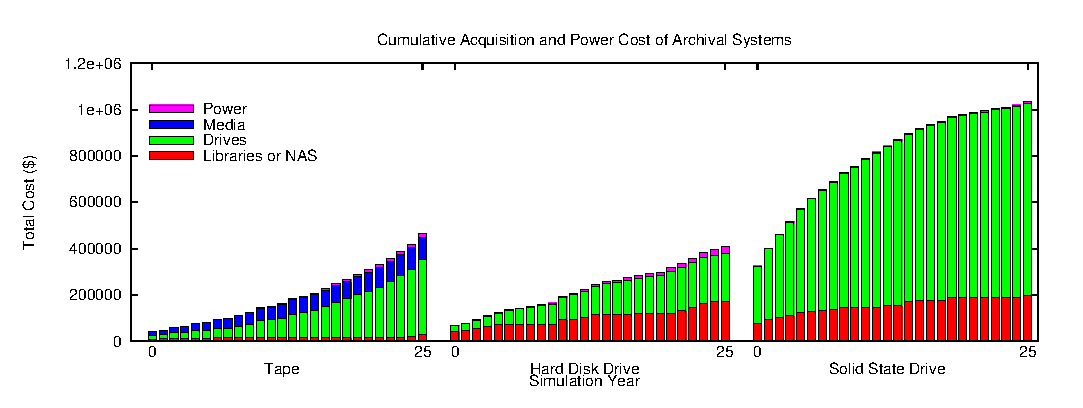
\includegraphics[width=\linewidth]{fig1.eps}
\caption{Tape, hard disk, and solid state disk can be used in archival storage systems.  The cost of NAS devices significantly impacts the TCO for HDD-based archives.}
\label{fig1}
\end{figure*}

\subsection{NAS Node for Distributed Storage}
Based on the results of our previous simulation work, we proposed a simple, low-power, and low-cost network attached storage device that can connect individual hard drives to a network at a much lower cost than the comparatively high-cost and high-performance NAS solution that we used above~\cite{web35}.  The proposed storage node connects a single SATA hard disk to a network while consuming 10 watts of active power and 1 watt of power while idle.  These specifications are based roughly on the Banana Pi~\cite{web40}, but they could be extended to the functionally similar Raspberry Pi~\cite{web49} or similar device.

Figure~\ref{fig2} shows the cumulative acquisition cost of the low-cost NAS devices in an archival system over a 25 year simulation period compared with that of the high-performance NAS devices.  The lower cost of the simple and low-cost NAS device suggests that it may prove to be an attractive option for archival systems and all storage systems that prefer lower cost to high-performance.  Yet while the cost of using simple compute devices to connect HDDs and SSDs to a network can be determined empirically, the total power consumption of such devices under archival workloads may vary from the predictions of the simulator.  Furthermore, the amount of communication between the storage nodes can further impact the power consumption and reliability of the archival system.  The following sections present the implementation of a distributed storage system using simple storage nodes that are similar to those modeled in the simulator.  We describe the behavior and performance characteristics that we observed, and we describe strategies to increase redundancy while minimizing the amount of coordination between nodes.

\begin{figure}[!ht]
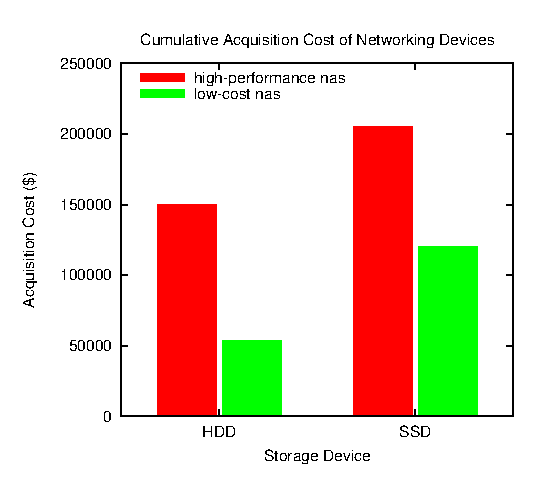
\includegraphics[width=\linewidth]{fig2.eps}
\caption{The cost of NAS devices in archival storage contributes to the total cost of ownership.  Lowering the cost of NAS devices by using a simple and low-cost compute device can help to reduce TCO.}
\label{fig2}
\end{figure}

\section{Implementation}
In this section, we describe the implementation of the storage system for archiving data on a distributed group of simple and low-power storage nodes.  We also describe the potential for further refinements to the communication and coordination between nodes to increase redundancy, including tradeoffs with cost, performance, and power consumption.

The source code of our archival storage prototype can be downloaded from \url{https://github.com/JamesByron/CMPS232-Spring18}.

\subsection{Storage Server Nodes}
We created a server application that runs on each storage node of the prototype archival storage system.  The server application uses a hard disk that is connected to the node to store data that it receives over a network.  Storage nodes spend most of their time in an idle state when waiting to receive a message over the network to store, retrieve, or verify files on its hard disk.  We have implemented support for file storage and verification in our prototype.  File retrieval is left for future work, and we expect its design to mirror that of the file storage service.  Storage nodes record a list of the files that they have received and the checksums of those files in order to later verify their correctness.

\subsubsection{Storage Node Configuration and Idle State}
Each node is assigned a static IP address, and we assign consecutive IP addresses to the nodes in our prototype so that clients and other nodes can easily detect which nodes are available when looking for a location to store data or to perform any other action on the network.  Program files are stored locally on each node in its on-board Flash storage, separately from the archival data on the hard disk.  We also store the checksums of archived files on the boot drive of each storage node.

The idle state for a storage node begins when the node boots and initializes itself as a member of the archival storage system.  The hard drive connected to the node is spinning by default at the time of boot.  The node reads from the drive and calculates how much free space is available on it.  This value is reported to any client that contacts it to stored data.  Next, the node unmounts the hard drive and spins down the hard drive.  Finally, the storage node awaits a connection from a client over the network to begin receiving data or verifying file contents.

\subsubsection{Receiving Data}
When a node receives data for it to add to the archival system, it first receives a connection from a client over the network.  Next, the node mounts and spins-up the hard disk that is connected to it.  The mounting can take several seconds.  When complete, the storage node reports its available capacity to the client through the network.  The client is responsible for knowing the size of the files that it is storing and to select a storage node that has enough free capacity to store the data.  The node logs the time at which a socket connection was opened with a client.  The storage node parses the first packet of data from the client to find the file name that it should use to store a file.  If the file already exists on the node's hard disk, the old file is simply replaced, and the checksum for the new file will replace the old checksum.  We choose to replace old files rather than to create a second version because the client may need to replace a file that was originally corrupted during transmission.  The node continues to receive packets of data until the end of the file.  If the client has more files to store, it begins transmitting a new file to the storage node.  When the server node has finished receiving data, it receives a termination message from the client through the network and unmounts the hard disk.  The hard disk spins down within a few seconds to save power.

\subsubsection{Verifying Data}
Each server node has sufficient processing power to verify or scrub the files that it stores.  This is an important advantage of the prototype archival system using simple compute devices.  Verification begins with each node reading the contents of the file list that it stores.  Next, the node computes a hash of each file on the hard disk, checking the hash against the checksum that is stored in the file list.  The results of each comparison are stored in a log file on the storage node.  Figure~\ref{fig3} shows a diagram of the prototype that we have implemented with data and hashes stored as checksums on the internal storage of each node.

\begin{figure}[!ht]
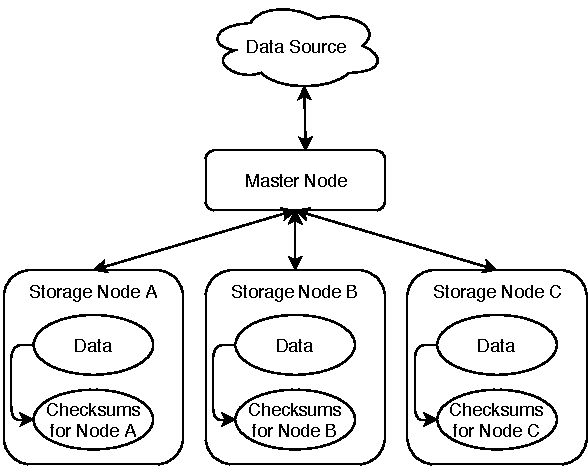
\includegraphics[width=\linewidth]{fig3.pdf}
\caption{The design of our prototype stores data and checksums on each node.  Communication is performed between the client (master) node and the storage (server) nodes.}
\label{fig3}
\end{figure}

\subsection{Storage Client}
The client application is responsible for finding a storage node that has sufficient capacity to store the data that it needs to store.  We assume that the client knows nothing about each server node except which IP addresses the servers are assigned to.  Clients also operate with the same communication protocol as the server when receiving the available capacity of a server and sending file names and data to the server.   The client contacts each node sequentially until a server is found that has sufficient capacity to store the data.  The client sends the contents of the files to store them into the archival system.

In addition to the transmission of data, clients can also send messages to each server to reboot a server, shutdown a server, reset a server and erase all its data, upload a new version of the prototype archival software to it, or initialize the server to receive data.

\subsubsection{Challenges in Coordination}
We experienced a challenge during the testing of our prototype that implicated the coordinated communication between server and client.  We initially chose to perform a checksum of each file received by a server when the transmission from client to server completed.  With most files, the checksum process completed quickly because the file size was small.  In some cases, however, the file size of several gigabytes caused the checksum to take several minutes.  During this time, the connection between client and server could time out, resulting in a communication error that required the restart of the receive application in the server.  We removed the verification operation during file transmission and found that the communication problem no longer occurred in our experiments.  We may revisit this error at a later time to explore alternative techniques to create checksums for a file at the time the file is received without causing lengthy network delays.

\begin{figure}[!ht]
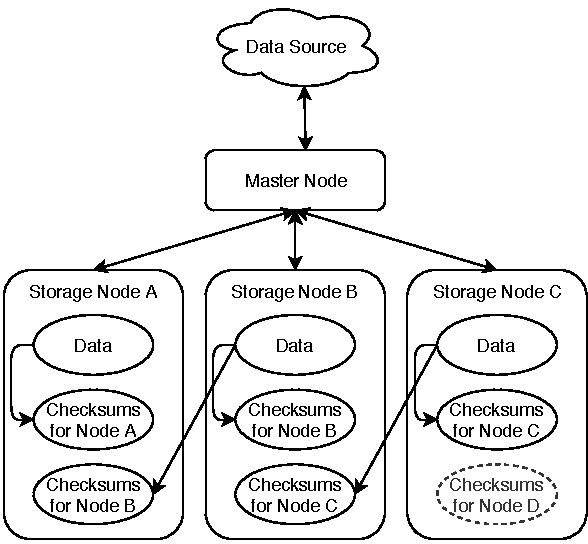
\includegraphics[width=\linewidth]{fig4.pdf}
\caption{Potential communication between nodes can share information about their checksums.}
\label{fig4}
\end{figure}

\subsection{Duplication of Checksums for Verification}
Here we present some design optimizations that will likely improve the performance of our prototype.  In our initial design, we implement a simple client-to-server model that relies on communication between each server and a client to report capacity.  Checksums to verify the correctness of each file on each node are also stored only on the node that also stores the corresponding files.  Figure~\ref{fig4} present a modified implementation that records the checksum information for each node on the node that stores the data and also on its neighbor.  In this design, the neighbor to the left joined the storage system at the same time or before the node on the right.  New nodes added on the right may locate an older node to the left to store a copy of its checksum data.  Data may also be duplicated in this way.  The advantage of such a design would be that each node is aware of the files that are stored on other storage nodes, thereby reducing the number of server nodes that a client would have to contact in order to locate a file.  Copying checksum or file data between nodes will inevitably increase the communication and coordination between nodes and the power that they consume.  Nevertheless, we regard this as an important improvement to make for future work in order to ensure the durability of data in the archival system.

\section{Experimental Setup}
We ran our experiments with a group of three Raspberry Pi 3 B + computers~\cite{web49}.  The nodes are connected to one hard disk each.  The hard disks that are attached to the three nodes are 250GB, 500GB, and 1TB, respectively.  We also use a gigabit Ethernet switch to connect the three Raspberry Pis to a network.  Our client computer connects to the switch through its own gigabit Ethernet connection.

\subsection{Archival Data}
We use a combination of data to be stored in our archival system.  File sizes range from less than 100 bytes to more than 10GB.  Figure~\ref{fig5} shows the distribution of the number of files by size that we store using the prototype.  All our experiments were executed once, and we average the results of any files that share the same category for size.  We verify the data in the archival system once, measuring the time to complete the verification on each node and also the total power consumption.

\begin{figure}[!ht]
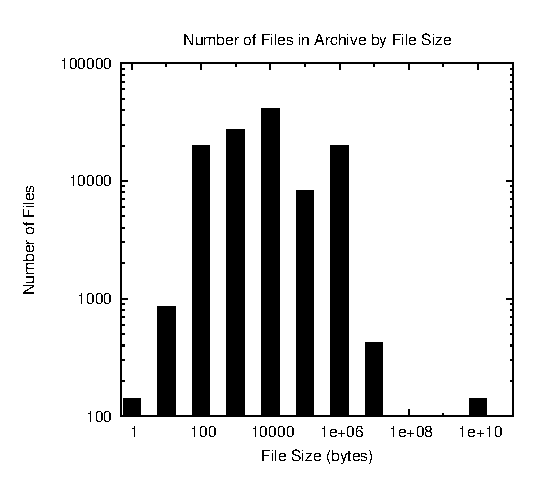
\includegraphics[width=\linewidth]{fig5.eps}
\caption{The number of files by file size in the archival dataset allows us to gather data on performance and communication overhead using a diverse workload.}
\label{fig5}
\end{figure}

\subsection{Measuring Instrumentation}
We measure the amount of data transmitted, time taken, and total data stored on the storage server nodes and also on the client.  We measure the electricity consumption using a  P3 International P4460 Kill-A-Watt EZ Electricity Monitor, which reports the total kilowatt hours that our prototype consumed during our experiment.

\subsection{Simulator Setup}
We configure our simulator to simulate the use of 250GB, 500GB, and 1TB hard drives when increasing capacity.  The simulator uses one of each type of hard drive to simulate the effect of adding capacity with larger hard drives over time.  We consider the total active time from the simulator and compare it with our observed active time from the prototype.  As with our experiments using the prototype, the simulator will record the active time to write all data into the storage system and also to verify or scrub the data once.

We configure the simulator to use parameters that reflect the behavior of the Raspberry Pis and hard drives.  The Raspberry Pi provides USB 2.0 connectivity for each hard drive, and we therefore limit the throughput of each hard drive to 20 MB per second in the simulator.  This performance is significantly less than each HDD’s performance over SATA, and we expect the slower performance to increase total power consumption it our simulations.  The throughput also does not grow during the simulations.  We use the typical power consumption of hard drives similar to those in our prototype~\cite{web50,web38}.  We configure the simulator to scrub the data once during the simulation as we do with the prototype.

\section{Experimental Results}

\subsection{Prototype and Simulation}
We first compare the results of the power consumption and time taken for our prototype to archive data with the results of our simulation.  Table~\ref{tab:comp} shows a summary of our findings.  The values for \textit{real time} and \textit{real power} are taken from the prototype archival system, and the \textit{sim power} and \textit{sim time} are taken from the simulation.  We observe that the real time taken and power consumption are both greater than the predictions from the simulator.  The variance is greatest at the end of the simulation, when the power use increases by 0.18 kWh while the prototype increases by 0.79 kWh.  We identify several possible factors that may contribute to the growth of the difference between the prototype and simulated results between the second and third simulation period.

\begin{table*}[!hbt]
\begin{minipage}{\linewidth}
\centering
  \caption{Storage Media Parameters}
  \label{tab:comp}
  \begin{tabular}{lr|rr|rr}
    \toprule
    \textbf{Period}&\textbf{Capacity}&\textbf{Sim. Time}&\textbf{Sim. Power}&\textbf{Real Time}&\textbf{Real Power}\\
    \midrule
    1&250 GB&192 min&0.05 kWh&210 min&0.06 kWh\\
    2&500 GB&518 min&0.14 kWh&600 min&0.19 kWh\\
    3&1 TB&1170 min&0.32 kWh&1435 min&1.1 kWh\\
  \bottomrule
\end{tabular}
\end{minipage}
\end{table*}

Our simulator reports a throughput of 60 MB/second at the end of the simulation.  Each node offers a 20 MB/second bandwidth for its own data, so the report from the simulator is accurate.  Nevertheless, when writing data to the archival system, the total bandwidth never exceeds 20 MB per second because only the newest drive has available capacity to store more data.  Thus the effective throughput of the archival system remains 20 MB per second.  By using the higher value of 40 MB per second of bandwidth when there are two active storage nodes and 60 MB per second when there are three active storage nodes, the simulator predicts that it will take less time to write additional data to the archive.  It also underestimates the time taken to scrub the data on the hard disks, since the smallest hard disk has to read only 250 GB at 20 MB per second while the largest hard drive must read 1 TB at the same speed.  The simulator assumes for the sake of simplicity that the combined speed of the hard drives can be applied to the data stored on each particular drive, thereby underestimating the amount of time required to  write and verify data.

Our simulator has been designed to regard the behavior of archival storage systems as a whole rather than as individual drives storing individual files.  The results of this experiment suggest that, in order to improve the predictions of the power consumption of an archival system, we should implement a model that tracks the specific capacity and contents of individual storage devices to record how the archive's workload affects them individually.  We may then determine the performance of the archival system as a whole by determining the aggregate behavior of all of its storage devices separately.

An additional factor that likely affects the power consumption of the prototype simulator differently than the simulation is that we do not consider the power consumption of the network switch in our simulation.  We did not expect the network switch to consume a significant amount of power; however, the power consumption of networking may also increase the power consumption of the prototype relative to the simulation in our experiment.

\subsection{File Size and Transfer Speed}
We measured the transfer speed while storing data into the archival nodes.  Each File transfer begins with an initial packet that contains the file name that the storage node should use to store the newly archived file.  The node then receives data in 4 KB packets until the end of the file.  We expected that the transfer speed would show an increase with larger files because the time needed read and parse the first packet of data would be distributed over many packets rather than a few.  The average file transfer speed by file size is shown in Figure~\ref{fig6}.  We observe an overall trend that large files promote faster file transfers.  Surprisingly, however, files of moderate size transferred much more quickly than the largest files.  The maximum throughput of the USB interface that each of our HDDs communicates with is roughly 20 MB per second, as observed with the largest file size here.  We saw a maximum throughput of approximately 120 MB per second for files around 20 KB.  120 MB per second is also the maximum bandwidth of the gigabit Ethernet connection that we use in our experiments.

\begin{figure}[!ht]
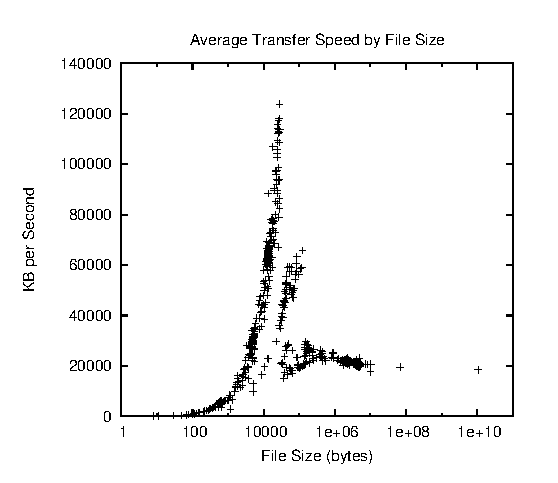
\includegraphics[width=\linewidth]{fig6.eps}
\caption{The file transfer speed incrreases for larger files.  We observed transfer speeds above the maximum speed of the USB interface for files around 20 KB in size.  The peak file transfer speed matches the maximum throughput of the gigabit Ethernet switch.}
\label{fig6}
\end{figure}

The high throughput of files that are around 20 KB may be explained as a feature of OS-level caching.  Operating systems like Linux provide some caching for data as user-space applications interact with the file system, so the high throughput for some files may reflect a sweet spot between the efficiency of repeated data transfers and the speedup of OS-level caching for files up to a certain limit in size.  Larger files don't fit in the main memory of the Raspberry Pi, so large files must inevitably be written to disk as the storage node receives them.

\subsection{Communication and File Transfer Time}
Figure~\ref{fig7} shows the efficiency of file transfers into the archival system by file size.  We expect that larger files will provide greater efficiency than smaller files because the performance cost of establishing a network connection, parsing the first data packet, and creating a new file can be amortized over more data packets without interruption.   A value of 1 represents a high degree of transfer efficiency.  We observe that file transfers become increasingly efficient as the file size increases.  Some files do not fit the dominant curve of efficiency increasing by file size.  There are several possible reasons for such outliers.  When a node reads the first packets of data from a client over the network, it can take several seconds to establish a connection and begin archiving data.  This can, for such cases, result in lower transfer efficiency.  Also, the performance of hard drives can vary in unpredictable ways due to logic that runs internally on the drive itself.  We expect that a combination of these two factors causes the variance of the data in Figure~\ref{fig7}.

\begin{figure}[!ht]
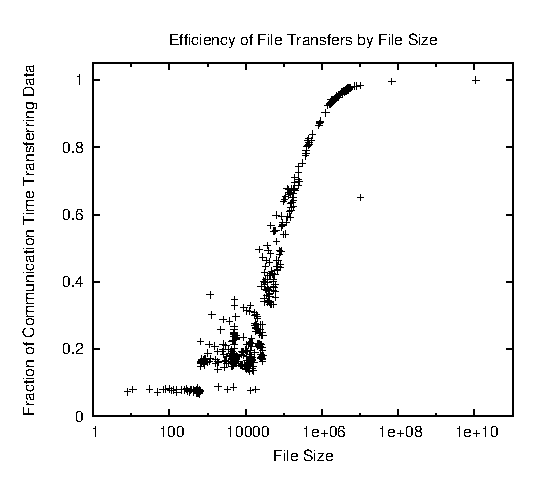
\includegraphics[width=\linewidth]{fig7.eps}
\caption{We calculate file transfer efficiency by dividing the file transfer time by the total time needed to archive a file.  Efficency increases as the file size grows, thereby illustrating the overhead of negotiating a network connection and creating a file on the storage node.}
\label{fig7}
\end{figure}

\subsection{Verification Performance}
We measured the time taken to verify the files in the archival system once they were written onto the storage devices.  In Figure~\ref{fig8}, both axes are logarithmic.  We observe that the time taken to verify a file grows roughly linearly with the size of the files.  As with other experiments, there is some variance with smaller files because the time needed to read a small file may be no smaller than the time needed to read a file that is slightly larger.  Hard drives read blocks of data in chunks of several KB, so small files require the hard drive to read much more data than necessary.  The linear growth of verification time shows the benefit of using low-power compute devices to connect an HDD to a storage network.  The storage node can verify files because it has sufficient computation power, and the data does not need to be transmitted over the network to a different server for verification, thereby reducing the number of data transfers and coordination between storage nodes or servers.

\begin{figure}[!t]
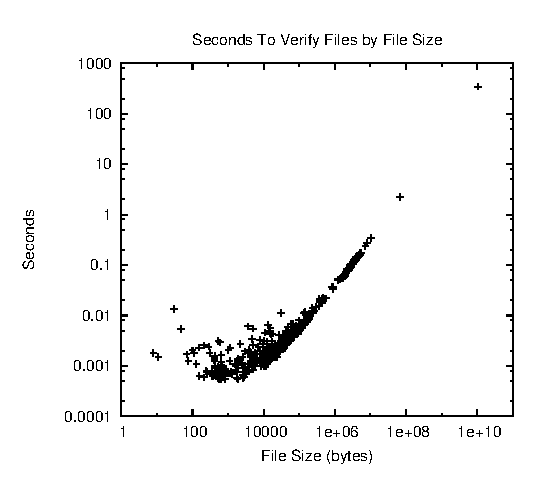
\includegraphics[width=\linewidth]{fig8.eps}
\caption{In general, file verification takes longer for larger files.  The results are highly variable for small files, even taking longer for some small files than for larger files.  The axes here are logarithmic.}
\label{fig8}
\end{figure}

\section{Conclusion}
We have presented the design and implementation of a prototype distributed archival storage system that implements the simple storage node that we model with our archival simulator.  We found that the energy consumption in our prototype exceeds the energy consumption that we predicted in our simulator.  We describe several factors that contribute to the difference.  We also described the cost of network coordination and overhead for the nodes in our prototype storage system.  We found that communication and coordination between a client and a server significantly affects the total performance of the storage system.  We defined several areas for future work that could improve both our prototype and the simulation model.
